% --------------------------------------------------------------------------------------------------
% Section: Preventive Measures
% Overview: Discusses strategies to prevent lung cancer, primarily through risk reduction methods.
% --------------------------------------------------------------------------------------------------

\section{Preventive Measures}

% Introductory paragraph about prevention strategies
The most effective strategies to prevent lung cancer focus primarily on reducing exposure to known 
risk factors, especially tobacco smoke, and minimizing contact with environmental and occupational 
carcinogens.

% --------------------------------------------------------------------------------------------------
% Subsection: Smoking Cessation Programs
% Focuses on benefits, success rates, and components of quitting smoking
% --------------------------------------------------------------------------------------------------

\subsection{Smoking Cessation Programs}

% Benefits of quitting even after a lung cancer diagnosis
There are many studies, mostly retrospective, which suggest that quitting smoking after a diagnosis 
of lung cancer may be associated with significantly decreased mortality \cite{20093278}, 
postoperative complications, recurrence and incidence of second primary lung cancer. In addition, 
there might be greater treatment effectiveness and quality of life \cite{22244802}. Tobacco smoking 
cessation interventions play an important role in the management of people with cancer.

% General benefits of cessation for prevention and overall health
Smoking cessation programs offer numerous significant benefits, including a substantial 
\textbf{reduction in mortality risk}, particularly when combined with lung cancer screening, which 
greatly lowers the chances of death from lung cancer and related comorbidities. These interventions 
also contribute to \textbf{increased life expectancy}, with more life-years gained. Beyond lung 
cancer, quitting smoking improves \textbf{overall health} by decreasing the risk of various 
diseases. For individuals who have been treated for lung cancer, cessation \textbf{reduces the 
likelihood of developing new lung cancers}. 

% Effectiveness and success rate data for cessation programs
\begin{itemize}
    \item \textbf{Effectiveness and Success Rates:}
        \begin{itemize}
            % Quit rates decrease over time
            \item \textit{Success rates vary over time:} Quit rates tend to decline as time from 
            quitting increases. For example, one study reported quit rates of 88.2\% at 4 weeks, 
            54\% at 6 months, and 36\% at 12 months after cessation. \cite{37297676} Another study 
            showed a 45.3\% abstinence rate at one year in a smoking cessation clinic setting. 
            \cite{Esen2020}

            % Multimodal treatment yields better results
            \item \textit{Combination therapy is most effective:} Programs that combine behavioral 
            counseling with pharmacological treatments (like nicotine replacement therapy, 
            varenicline, or bupropion) show higher success rates (24\% at one year) compared to 
            behavioral support alone (7\%-16\%) or no structured intervention (3\%-5\%). 
            \cite{cureus2024}

            % Tailored, interdisciplinary care improves long-term outcomes
            \item \textit{Individualized, multidisciplinary approaches improve outcomes:} 
            Incorporating psychiatric and psychological consultations, counseling, education, and 
            medication tailored to the individual’s needs increases quit rates, sometimes reaching 
            up to 40-45\% at one year in specialized clinics. \cite{37297676}
        \end{itemize}
\end{itemize}

% Smoking cessation methods image
\vspace{1em}
\begin{center}
    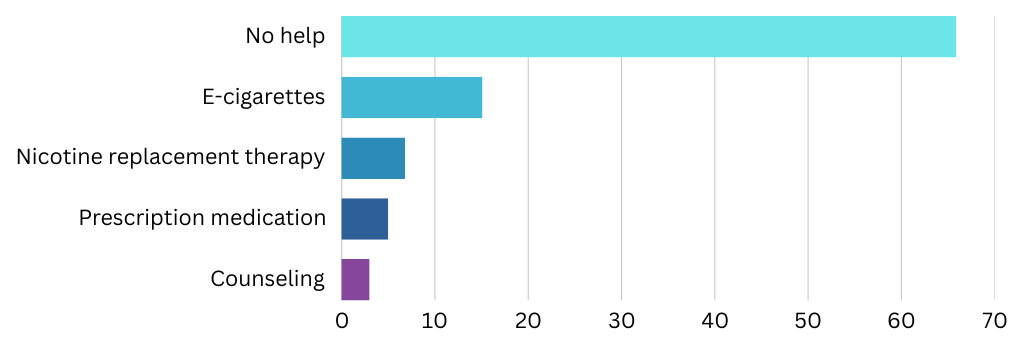
\includegraphics[width=\textwidth]{../assets/06-prevention/smoking-cessation.png}

    \small\textit{Percentages using different smoking cessation methods. Data source: 
    \cite{who2018}}
\end{center}
\vspace{1em}

% Components of effective cessation programs
\begin{itemize}
    \item \textbf{Components of Smoking Cessation Programs:}
        \begin{itemize}
            % Psychological support tools
            \item \textit{Behavioral Counseling:} Includes motivational interviewing, cognitive-
            behavioral therapy, and psychoeducation to address psychological dependence and 
            triggers.

            % Medications to help with nicotine withdrawal
            \item \textit{Pharmacotherapy:} Medications such as nicotine replacement therapy 
            (patches, gum), varenicline, and bupropion help reduce withdrawal symptoms and cravings.

            % Long-term monitoring for relapse prevention
            \item \textit{Follow-up and Support:} Regular follow-up visits or remote support 
            (phone, telemedicine) improve long-term abstinence by providing ongoing encouragement 
            and relapse prevention. \cite{Esen2020}
        \end{itemize}
\end{itemize}

% --------------------------------------------------------------------------------------------------
% Subsection: Early Screening and LDCT
% Explanation and importance of low-dose CT scans in early detection
% --------------------------------------------------------------------------------------------------
\subsection{Early Screening and LDCT}

% Overview of LDCT and its operation
\textbf{Low-dose computed tomography (LDCT)} is a specialized imaging procedure that uses a low 
dose of radiation to produce detailed, high-quality pictures of the lungs, allowing for the 
detection of small lung nodules and early-stage lung cancer. The scan is quick, non-invasive, and 
involves lying on a table while an X-ray machine rotates around the chest to capture multiple 
images, which are then combined into 3D views of the lungs. 

% Screening recommendations and effectiveness
LDCT is the \textit{only recommended screening test for lung cancer}, particularly for high-risk 
individuals such as current or former smokers aged 50 to 80 with a significant smoking history (20 
pack-years or more). Lung cancer is often asymptomatic in early stages, leading to late diagnosis 
and poor outcomes. The key benefit of LDCT screening is its ability to reduce lung cancer mortality 
by about 20\% by detecting cancer early when treatment is more effective and survival rates are 
significantly higher. Although LDCT involves some radiation exposure, it is much lower than standard 
CT scans, making it a safer option for annual screening. \cite{sl2020}

% Importance for improving treatment success
Early detection through LDCT enables less invasive treatments and improves patient outcomes, making 
it a crucial tool in lung cancer prevention and management.

% --------------------------------------------------------------------------------------------------
% Subsection: Public Health Education
% Educational strategies for reducing lung cancer incidence
% --------------------------------------------------------------------------------------------------
\subsection{Public Health Education}

% Role of education in prevention
Public health education plays a crucial role in lung cancer prevention by increasing awareness about 
risk factors, promoting healthy behaviors, and empowering individuals to make informed decisions. 
Educational initiatives target various audiences, employing diverse strategies to maximize reach 
and impact.

% Key content areas for education programs
\textbf{Key areas to focus on in public health education} for lung cancer prevention include 
emphasizing the critical importance of \textbf{avoiding tobacco use and exposure to secondhand 
smoke}, as smoking is the leading cause of lung cancer and accounts for 80\% to 90\% of cases. 
Education should also \textbf{raise awareness about radon exposure}, encouraging home testing and 
mitigation to reduce this significant environmental risk factor. Additionally, \textbf{informing 
workers and employers} about minimizing occupational exposures to known carcinogens such as 
asbestos, arsenic, nickel, and chromium is essential. \textbf{Promoting healthy lifestyle choices}, 
including balanced diets and regular physical activity, may also contribute to lowering risk, 
although their direct effect on lung cancer prevention is less clear. Finally, public health efforts 
should \textbf{support smoking cessation programs} and enforce smoke-free environments to reduce 
both active and passive smoking risks, thereby decreasing lung cancer incidence and mortality. 
\cite{nci2025}

% Delivery channels for educational content
\vspace{1em}
\textbf{Delivery Methods for Public Health Education:}
\begin{itemize}
    \item Mass media campaigns using television, radio, and the internet to disseminate information 
    about lung cancer prevention.
    \item Community-based programs in schools, workplaces, and healthcare settings to provide 
    targeted education and support.
    \item Educational materials such as brochures, fact sheets, and websites to offer accessible 
    information about lung cancer risk factors and preventive measures.
    \item Healthcare provider education to ensure that doctors and other healthcare professionals 
    can effectively counsel patients about lung cancer prevention.
\end{itemize}

% Closing remark
By implementing comprehensive public health education strategies, communities can empower 
individuals to adopt healthier behaviors, reduce exposure to risk factors, and ultimately lower the 
incidence and mortality of lung cancer.
